\section{Progettazione Architetturale}
\textit{Dal 2021-01-18 al 2021-03-08}


\begin{figure}[H]
	\centering
	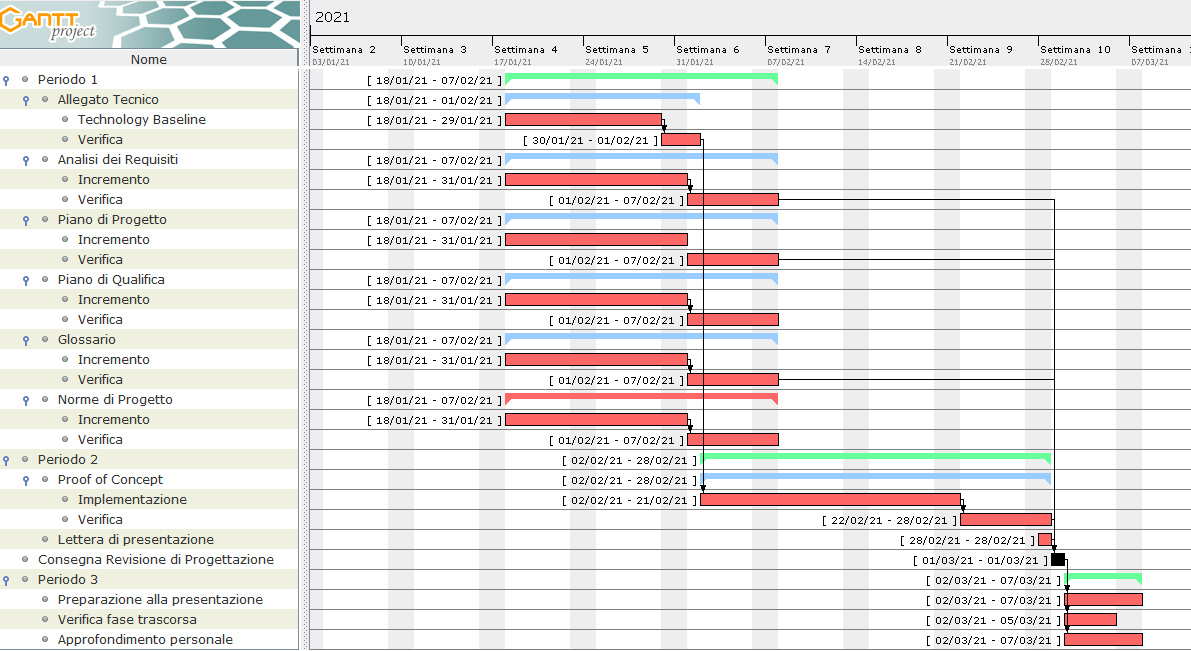
\includegraphics[scale=0.48]{res/images/gantt_fase/03_gantt_progettazione.png}
	\caption{Diagramma di Gantt\textsubscript{G} relativo alla fase\textsubscript{G} di Progettazione Architetturale}
\end{figure}


\subsection{Periodo 1}

\subsubsection{Pianificazione preventiva}

\paragraph{Attività}
\subparagraph*{}

\planningTable{
	Incremento Analisi dei Requisiti & L'avanzamento nello sviluppo del prodotto chiarirà alcuni aspetti che nella fase\textsubscript{G} di Analisi risultavano oscuri, e potrebbe evidenziare delle criticità non inizialmente considerate. Se necessario, viene raffinata l'\textsc{Analisi dei Requisiti} & 8 & Analista
\tabularnewline 
Incremento Piano di Progetto & Il \textsc{Piano di Progetto} viene migliorato fornendo maggior dettaglio, oltre che integrato con il consuntivo del periodo trascorso & 7 & Responsabile
\tabularnewline 
Incremento Glossario & Viene integrato con nuovi termini & 1 & Responsabile
\tabularnewline 
Incremento Piano di Qualifica & Il cruscotto viene aggiornato con i dati rilevati sul periodo trascorso & 16 & Verificatore
\tabularnewline 
\caption{Pianificazione preventiva - Progettazione Architetturale - Periodo 1}
}

\paragraph{Preventivo}
\subparagraph*{}

\hspace{-1cm}
\begin{minipage}{.50\textwidth}
\smallPreventivoTable{
	Responsabile & 8 & 240\\ 
Verificatore & 16 & 240\\ 
Analista & 8 & 200\\ 
Amministratore & 0 & 0\\ 
Programmatore & 0 & 0\\ 
Progettista & 0 & 0\\ 
\hlinetable 
\textbf{Totale} & \textbf{32} & \textbf{680}\\ 
\end{tabular} 
\caption{Preventivo - Progettazione Architetturale - Periodo 1}
}
\end{minipage}
\hspace{1cm}
\begin{minipage}{.40\textwidth}
\begin{figure}[H]
	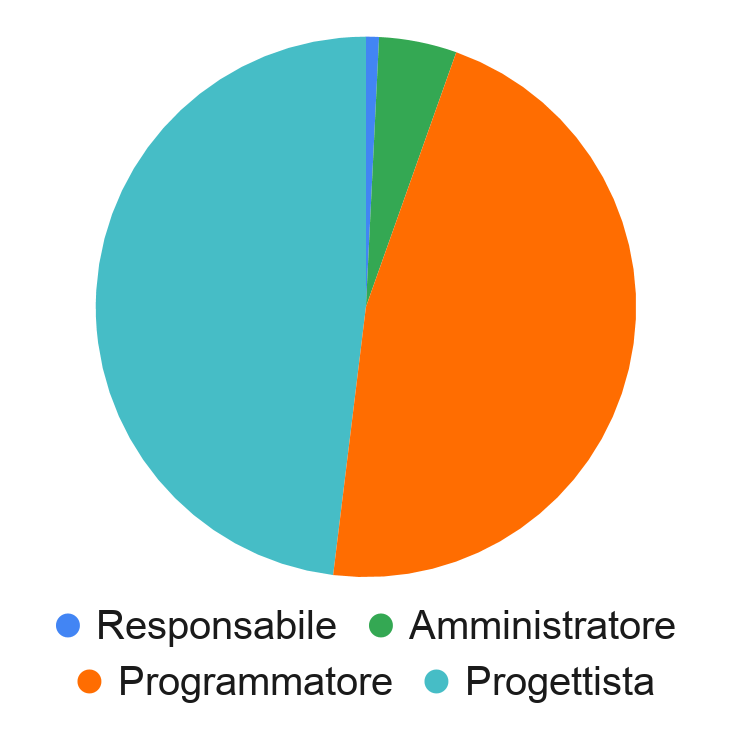
\includegraphics[scale=0.21]{res/images/charts/preventivo_priori/Grafico4-3.png}
	\caption{Distribuzione dei costi: preventivo - Progettazione Architetturale - Periodo 1}
\end{figure}
\end{minipage} 






\subsubsection{Pianificazione di periodo}

\begin{figure}[H]
	\centering
	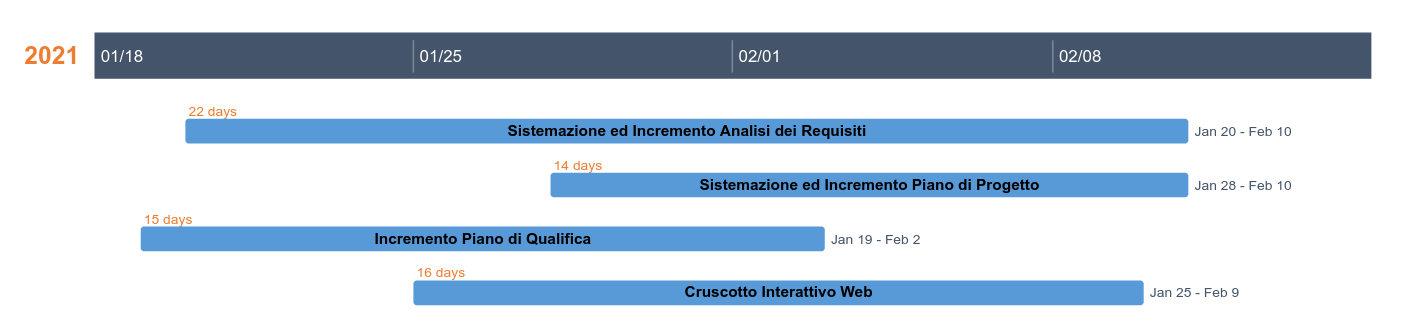
\includegraphics[scale=0.35]{res/images/gantt_periodo/progarch_1_gantt.png}
	\caption{Gantt di periodo\textsubscript{G} - Progettazione Architetturale - Periodo 1}
\end{figure}

\paragraph{Attività}
\subparagraph*{}

\planningTable{
	Sistemazione e incremento Analisi dei Requisiti & Nell'Analisi dei Requisiti viene fornito maggior dettaglio a dettagli non inizialmente approfonditi e vengono sistemate alcune criticità riscontrate.  & 8 & Analista
\tabularnewline 
Sistemazione e incremento \textsc{Piano di Progetto} & Il \textsc{Piano di Progetto} viene ristrutturato per rendere più fluente la consultazione e più guidata la pianificazione del progetto. Considerando il tempo risultato necessario a produrre la versione iniziale del documento, il monte orario sarà calibrato al rialzo. & 15 & Responsabile
\tabularnewline 
Incremento \textsc{Piano di Qualifica} & Il \textsc{Piano di Qualifica} viene arricchito e riorganizzato nella suddivisione delle metriche per facilitarne la consultazione. & 20 & Verificatore
\tabularnewline 
Cruscotto interattivo web & Viene predisposto un cruscotto interattivo che faciliti la visualizzazione immediata dell'andamento del progetto, con le nuove metriche presenti nel \textsc{Piano di Qualifica}. Essendo uno strumento nuovo, il monte ore viene stimato al rialzo.  & 10 & Verificatore
\tabularnewline 
\caption{Pianificazione di periodo\textsubscript{G} - Progettazione Architetturale - Periodo 1}
}

\paragraph{Preventivo orario ed economico}
\subparagraph*{}

\contabilitaTable{
	Chiarello Sofia & 0 & 0 & 4 & 0 & 0 & 0 & \textbf{4}\\ 
Crivellari Alberto & 0 & 12 & 0 & 0 & 0 & 0 & \textbf{12}\\ 
De Renzis Simone & 10 & 2 & 0 & 0 & 0 & 0 & \textbf{12}\\ 
Greggio Nicolò & 5 & 8 & 0 & 0 & 0 & 0 & \textbf{13}\\ 
Tessari Andrea & 0 & 8 & 0 & 0 & 0 & 0 & \textbf{8}\\ 
Zuccolo Giada & 0 & 0 & 4 & 0 & 0 & 0 & \textbf{4}\\ 
\hlinetable 
\textbf{Totale orario} & \textbf{15} & \textbf{30} & \textbf{8} & \textbf{0} & \textbf{0} & \textbf{0} & \textbf{53}\\ 
\textbf{Totale costo} & \textbf{450} & \textbf{450} & \textbf{200} & \textbf{0} & \textbf{0} & \textbf{0} & \textbf{1100}\\ 
\end{tabular} 
\caption{Preventivo di periodo - Progettazione Architetturale - Periodo 1}
}

\begin{figure}[H]
	\centering
	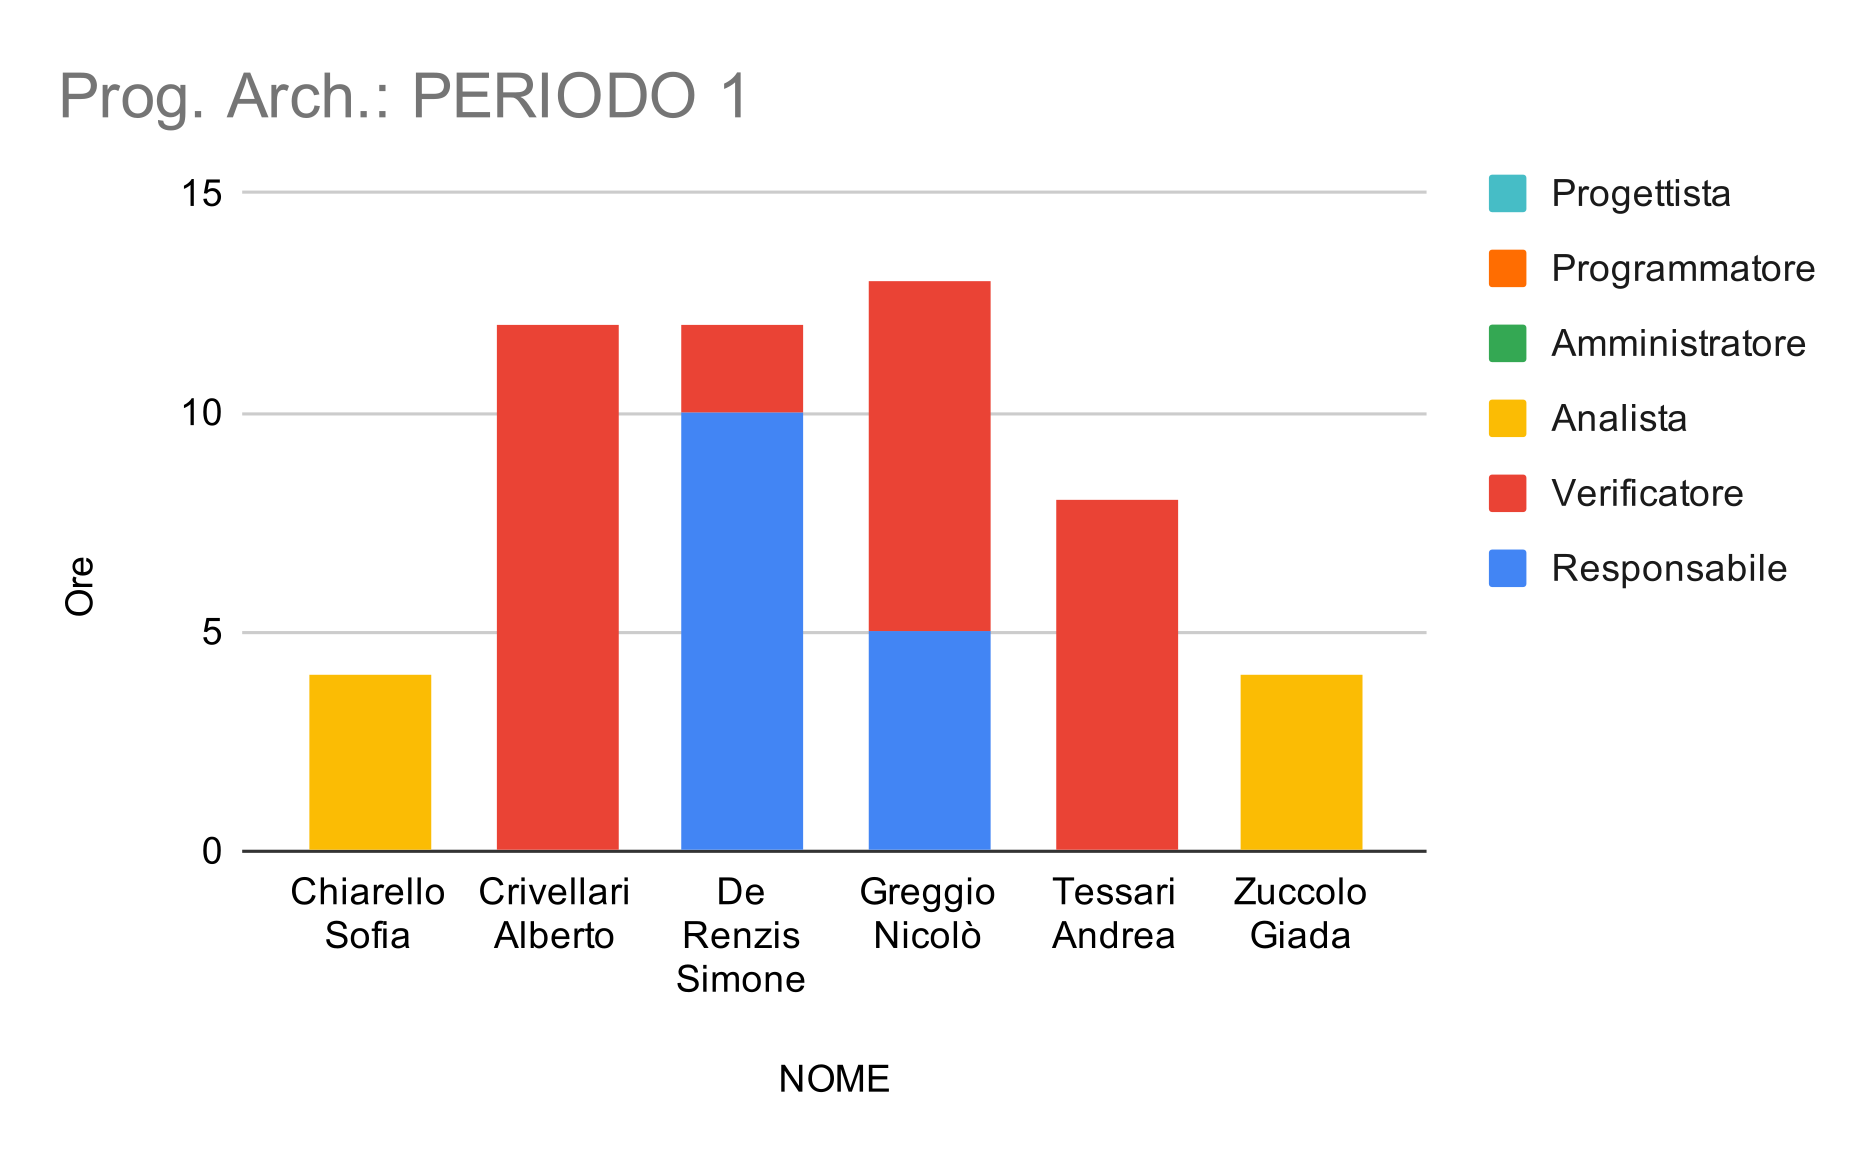
\includegraphics[scale=2]{res/images/charts/preventivo/prog_arch_1.png}
	\caption{Distribuzione oraria per componente: preventivo di periodo\textsubscript{G} - Progettazione Architetturale - Periodo 1}
\end{figure}


\subsubsection{Riscontro di fine periodo}


\paragraph{Consuntivo orario ed economico}
\subparagraph*{}

\contabilitaTable{
	Chiarello Sofia & 0 & 8 & 5 & 1 & 0 & 0 & \textbf{14} \\ 
Crivellari Alberto & 0 & 16 & 0 & 5 & 0 & 0 & \textbf{21} \\ 
De Renzis Simone & 13 & 6 & 0 & 4 & 0 & 0 & \textbf{23} \\ 
Greggio Nicolò & 9 & 4 & 0 & 5 & 2 & 0 & \textbf{20} \\ 
Tessari Andrea & 0 & 11 & 0 & 6 & 0 & 0 & \textbf{17} \\ 
Zuccolo Giada & 0 & 6 & 4 & 6 & 0 & 0 & \textbf{16} \\ 
\hlinetable 
\textbf{Totale orario} & \textbf{22} & \textbf{51} & \textbf{9} & \textbf{27} & \textbf{2} & \textbf{0} & \textbf{111} \\ 
\textbf{Differenza orario} & \textbf{7} & \textbf{21} & \textbf{1} & \textbf{27} & \textbf{2} & \textbf{0} & \textbf{58} \\ 
\textbf{Totale costi} & \textbf{660} & \textbf{765} & \textbf{225} & \textbf{540} & \textbf{30} & \textbf{0} & \textbf{2220} \\ 
\textbf{Differenza costi} & \textbf{210} & \textbf{315} & \textbf{25} & \textbf{540} & \textbf{30} & \textbf{0} & \textbf{1120} \\ 
\end{tabular} 
\caption{Consuntivo - Progettazione Architetturale - Periodo 1}
}

\begin{figure}[H]
	\centering
	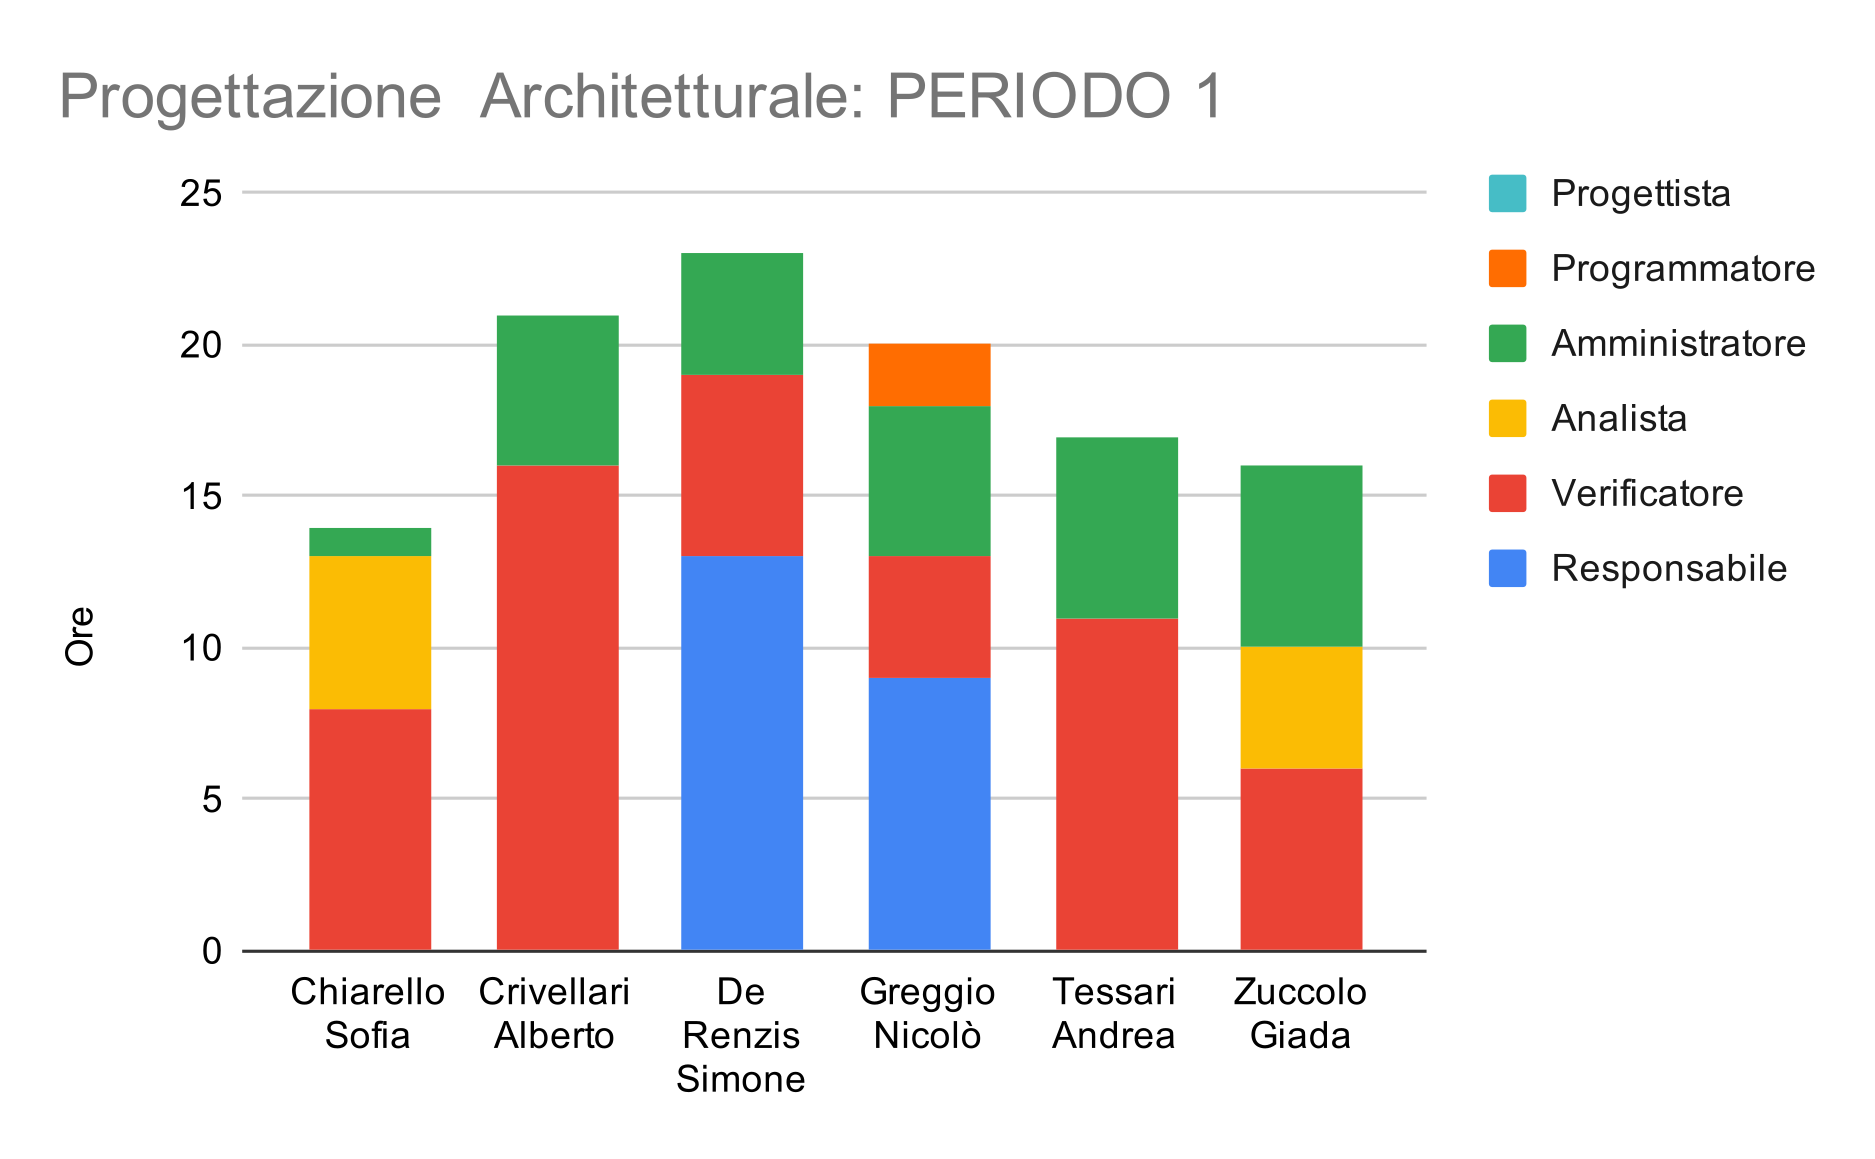
\includegraphics[scale=2]{res/images/charts/consuntivo/prog_arch_1.png}
	\caption{Distribuzione oraria per componente: consuntivo - Progettazione Architetturale - Periodo 1}
\end{figure}
\newpage
Il periodo\textsubscript{G} chiude in \textbf{negativo}, costringendo il gruppo ad una spesa supplementare di \textbf{1120 \euro} rispetto a quando preventivato all'inizio di questo periodo\textsubscript{G}. Rispetto a quando preventivato all'inizio del progetto\textsubscript{G}, il gruppo è in perdita di \textbf{1540 \euro}. Le ragioni di questo discostamento sono da ricercarsi nell'ampio lavoro di ristrutturazione resosi necessario a seguito delle criticità riscontrate nella Revisione dei Requisiti. In particolare, la realizzazione del cruscotto\textsubscript{G} interattivo e la riorganizzazione del \textsc{Piano di Progetto}, hanno richiesto molto tempo; questo investimento iniziale dovrebbe però assicurare una prosecuzione dei lavori più snella, risparmiando tempo nei periodi successivi.

\paragraph{Preventivo a finire}
\subparagraph*{}

\pafTable{
	Avvio & 1 & Consuntivo & 
\tabularnewline
Analisi dei Requisiti & 1 & Consuntivo & 
\tabularnewline
Analisi dei Requisiti & 2 & Consuntivo & 
\tabularnewline
Progettazione Architetturale & 1 & Consuntivo & 
\tabularnewline
Progettazione Architetturale & 2 & Preventivo di periodo\textsubscript{G} & 
\tabularnewline
Progettazione Architetturale & 3 & Preventivo & 280
\tabularnewline
Progettazione di Dettaglio e Codifica & 1 & Preventivo & 1270
\tabularnewline
Progettazione di Dettaglio e Codifica & 2 & Preventivo & 4097
\tabularnewline
Progettazione di Dettaglio e Codifica & 3 & Preventivo & 258
\tabularnewline
Validazione e Collaudo & 1 & Preventivo & 220
\tabularnewline
Validazione e Collaudo & 2 & Preventivo & 2145
\tabularnewline
Validazione e Collaudo & 3 & Preventivo & 60
\tabularnewline
\textbf{Totale} & \textbf{} & \textbf{} & \textbf{8330}
\tabularnewline
\textbf{Totale rendicontato} & \textbf{} & \textbf{} & \textbf{8330}
\tabularnewline
\caption{Preventivo a finire - Progettazione architetturale - Periodo 1}
}



\pagebreak
\subsection{Periodo 2}

\subsubsection{Pianificazione preventiva}

\paragraph{Attività}
\subparagraph*{}

\planningTable{
	Allegato Tecnico & Viene redatto l'\textsc{Allegato Tecnico}, nel quale viene presentata la Technology Baseline, ovvero l'architettura ad alto livello del software. & 62 & Progettista
\tabularnewline 
Setup ambienti di programmazione & Vengono organizzati e messi a punto i software e gli ambienti di sviluppo per i vari linguaggi impiegati. & 6 & Amministratore
\tabularnewline 
PoC - Incremento 1 & Una prima implementazione della soluzione permette di valutarne la bontà: viene realizzato un prototipo del software. Questo incremento riguarda la realizzazione backend del server. & 30 & Programmatore
\tabularnewline 
PoC - Incremento 2 & Realizzazione backend del'unità. & 5 & Programmatore
\tabularnewline 
PoC - Incremento 3 & Realizzazione frontend. & 15 & Programmatore
\tabularnewline 
PoC - Incremento 4 & Collegamento tra frontend e backend. & 10 & Programmatore
\tabularnewline 
Lettera di Presentazione & Avviene la stesura della lettera con cui il gruppo si candida alla Revisione di Progettazione. & 1 & Responsabile
\tabularnewline 
\caption{Pianificazione preventiva - Progettazione Architetturale - Periodo 2}
}

\paragraph{Preventivo}
\subparagraph*{}

\hspace{-1cm}
\begin{minipage}{.50\textwidth}
\smallPreventivoTable{
	Responsabile & 1 & 30\\ 
Verificatore & 0 & 0\\ 
Analista & 0 & 0\\ 
Amministratore & 6 & 120\\ 
Programmatore & 60 & 900\\ 
Progettista & 62 & 1364\\ 
\hlinetable 
\textbf{Totale} & \textbf{129} & \textbf{2414}\\ 
\end{tabular} 
\caption{Preventivo - Progettazione Architetturale - Periodo 2}
}
\end{minipage}
\hspace{1cm}
\begin{minipage}{.40\textwidth}
\begin{figure}[H]
	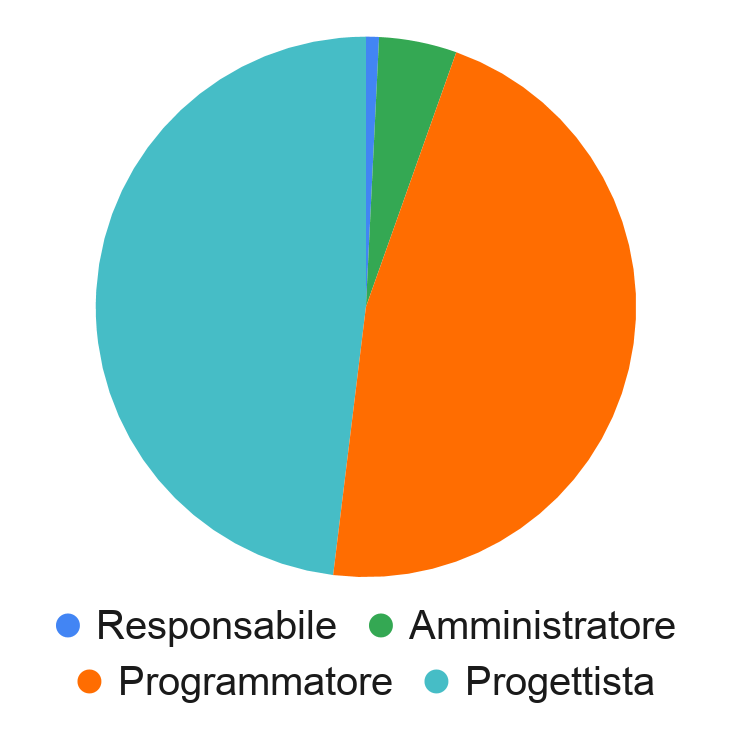
\includegraphics[scale=0.21]{res/images/charts/preventivo_priori/Grafico4-4.png}
	\caption{Distribuzione dei costi: preventivo - Progettazione Architetturale - Periodo 2}
\end{figure}
\end{minipage} 



\subsubsection{Pianificazione di periodo}

\begin{figure}[H]
	\centering
	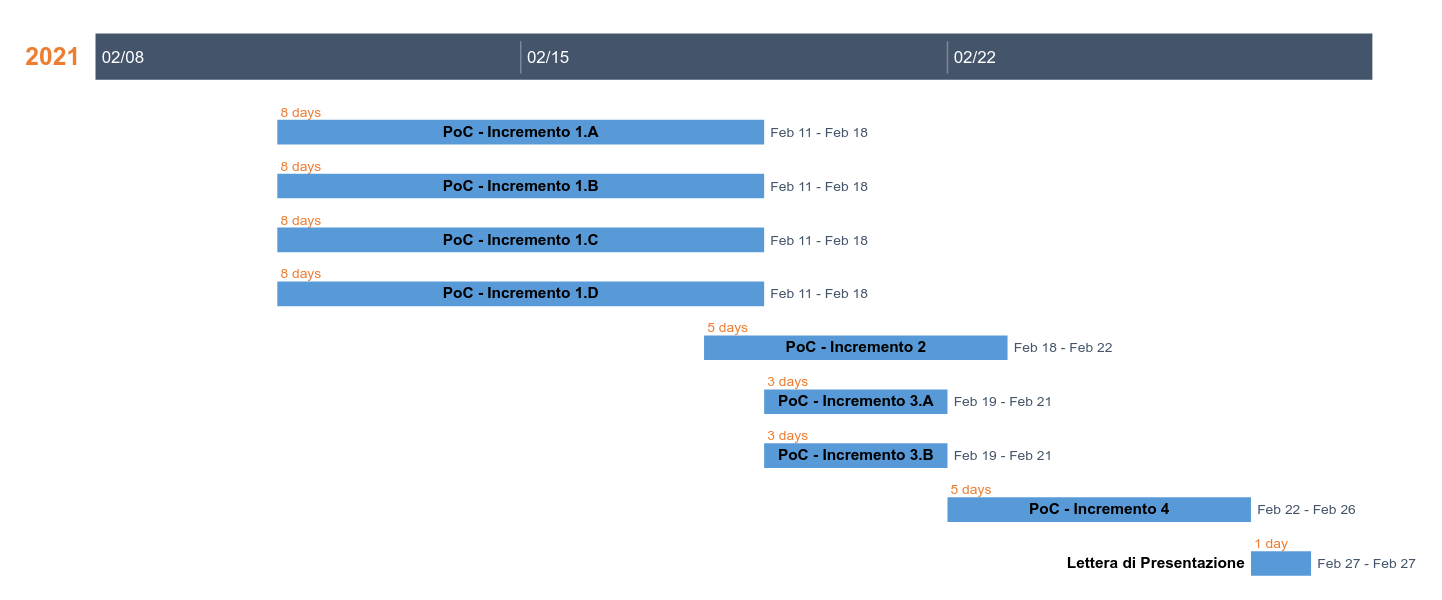
\includegraphics[scale=0.37]{res/images/gantt_periodo/progarch_2_gantt.png}
	\caption{Gantt di periodo\textsubscript{G} - Progettazione Architetturale - Periodo 2}
\end{figure}

\paragraph{Attività}
\subparagraph*{}

\planningTable{
	PoC - Incremento 1.A & Prima implementazione di studio per la comunicazione via socket tra le componenti in Node.js e il server in Java & 25 & Programmatore
\tabularnewline 
PoC - Incremento 1.B & Simulazione della mappa che visualizza le unità sulla base della posizione inviata dalle stesse & 15 & Programmatore
\tabularnewline 
PoC - Incremento 1.C & Definizione semplificata di un algoritmo per la ricerca del miglior percorso per raggiungere la destinazione & 5 & Programmatore
\tabularnewline 
PoC - Incremento 1.D & Ideazione e implementazione di sistema base per la rilevazione e gestione delle collisioni tra le unità & 25 & Programmatore
\tabularnewline 
PoC - Incremento 2 & Realizzazione del backend dell'unità in Node.js e collegamento con il server & 5 & Programmatore
\tabularnewline 
PoC - Incremento 3.A & Presentazione della mappa del magazzino tramite interfaccia realizzata in Angular.js & 20 & Programmatore
\tabularnewline 
PoC - Incremento 3.B & Aggiunta pannello di guida dell'unità nell'interfaccia grafica, e finestra di visualizzazione delle task\textsubscript{G} delle unità & 5 & Programmatore
\tabularnewline 
PoC - Incremento 4 & Collegamento tra server, frontend e unità & 20 & Programmatore
\tabularnewline 
Lettera di Presentazione & Avviene la stesura della lettera con cui il gruppo si candida alla Revisione di Progettazione & 1 & Programmatore
\tabularnewline 
\caption{Pianificazione di periodo\textsubscript{G} - Progettazione Architetturale - Periodo 2}
}


\paragraph{Preventivo orario ed economico}
\subparagraph*{}

\contabilitaTable{
	Chiarello Sofia & 0 & 0 & 0 & 0 & 20 & 0 & \textbf{20}\\ 
Crivellari Alberto & 0 & 0 & 0 & 0 & 20 & 0 & \textbf{20}\\ 
De Renzis Simone & 0 & 0 & 0 & 0 & 20 & 0 & \textbf{20}\\ 
Greggio Nicolò & 0 & 0 & 0 & 0 & 20 & 0 & \textbf{20}\\ 
Tessari Andrea & 0 & 0 & 0 & 0 & 20 & 0 & \textbf{20}\\ 
Zuccolo Giada & 1 & 0 & 0 & 0 & 20 & 0 & \textbf{21}\\ 
\hlinetable 
\textbf{Totale orario} & \textbf{1} & \textbf{0} & \textbf{0} & \textbf{0} & \textbf{120} & \textbf{0} & \textbf{121}\\ 
\textbf{Totale costo} & \textbf{30} & \textbf{0} & \textbf{0} & \textbf{0} & \textbf{1800} & \textbf{0} & \textbf{1830}\\ 
\end{tabular} 
\caption{Preventivo di periodo - Progettazione Architetturale - Periodo 2}
}

\begin{figure}[H]
	\centering
	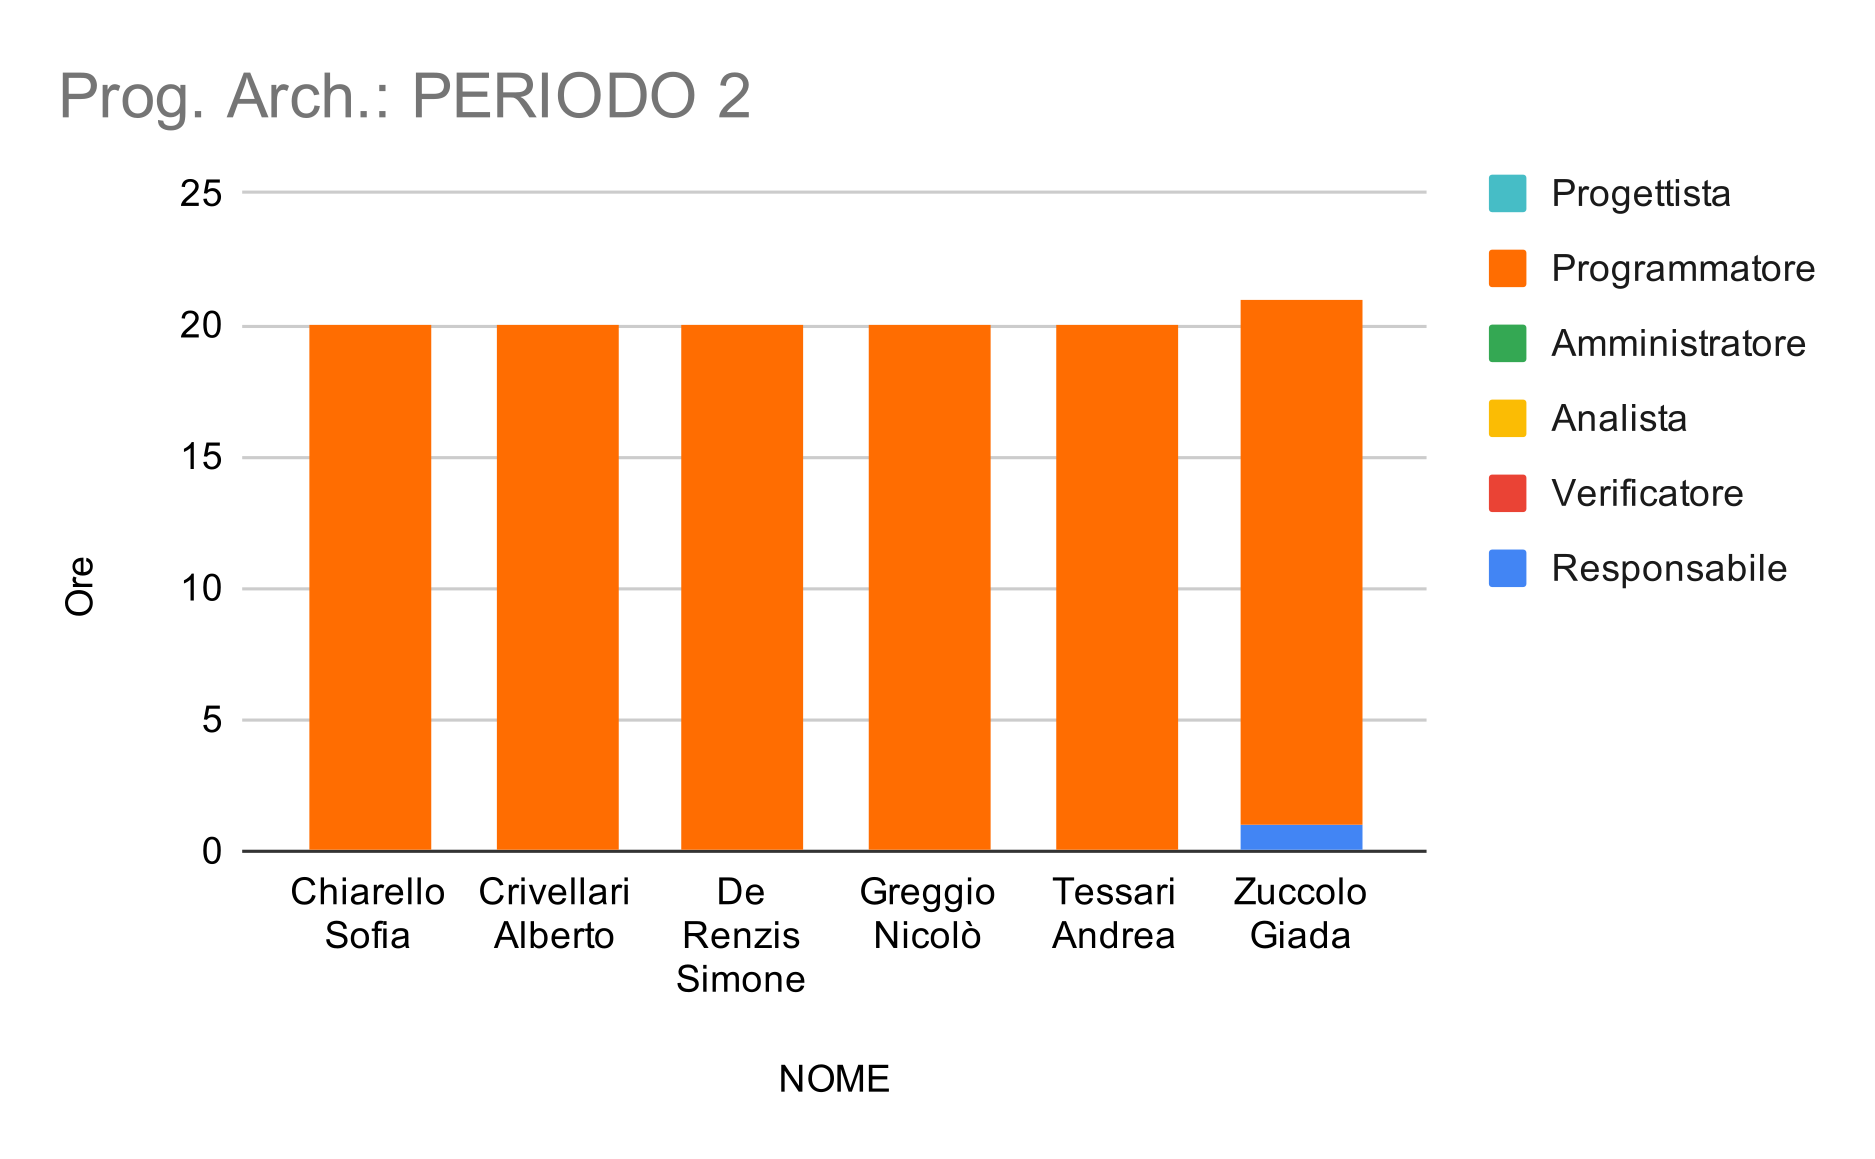
\includegraphics[scale=2]{res/images/charts/preventivo/prog_arch_2.png}
	\caption{Distribuzione oraria per componente: preventivo di periodo\textsubscript{G} - Progettazione Architetturale - Periodo 2}
\end{figure}

\subsubsection{Riscontro di fine periodo}


\paragraph{Consuntivo orario ed economico}
\subparagraph*{}

\contabilitaTable{
	Chiarello Sofia & 0 & 0 & 1 & 1 & 23 & 0 & \textbf{25} \\ 
Crivellari Alberto & 0 & 2 & 0 & 0 & 15 & 0 & \textbf{17} \\ 
De Renzis Simone & 0 & 0 & 0 & 0 & 18 & 0 & \textbf{18} \\ 
Greggio Nicolò & 0 & 0 & 0 & 1 & 20 & 0 & \textbf{21} \\ 
Tessari Andrea & 0 & 0 & 0 & 2 & 21 & 0 & \textbf{23} \\ 
Zuccolo Giada & 0 & 0 & 5 & 0 & 18 & 0 & \textbf{23} \\ 
\hlinetable 
\textbf{Totale orario} & \textbf{0} & \textbf{2} & \textbf{6} & \textbf{4} & \textbf{115} & \textbf{0} & \textbf{127} \\ 
\textbf{Differenza orario} & \textbf{-1} & \textbf{2} & \textbf{6} & \textbf{4} & \textbf{-5} & \textbf{0} & \textbf{6} \\ 
\textbf{Totale costi} & \textbf{0} & \textbf{30} & \textbf{150} & \textbf{80} & \textbf{1725} & \textbf{0} & \textbf{1985} \\ 
\textbf{Differenza costi} & \textbf{-30} & \textbf{30} & \textbf{150} & \textbf{80} & \textbf{-75} & \textbf{0} & \textbf{155} \\ 
\end{tabular} 
\caption{Consuntivo - Progettazione Architetturale - Periodo 2}
}

\begin{figure}[H]
	\centering
	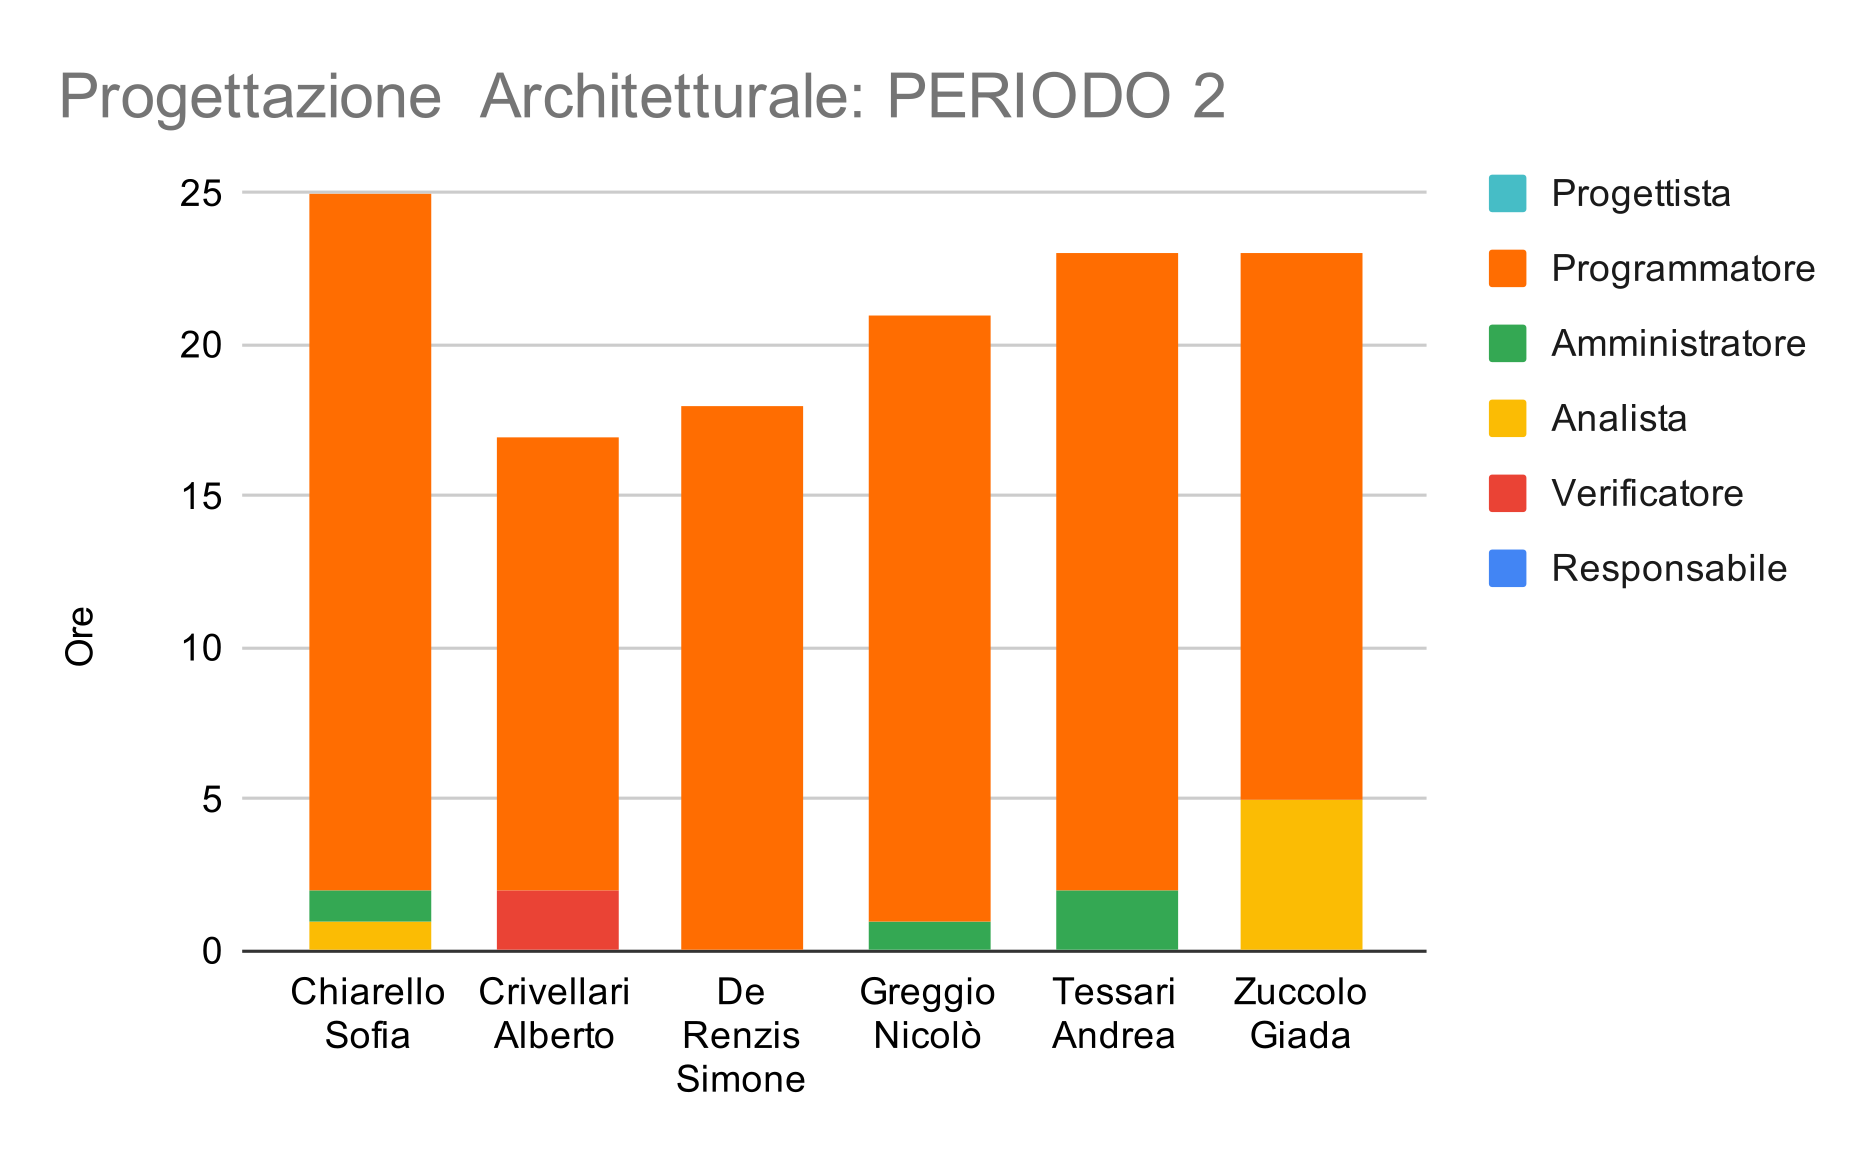
\includegraphics[scale=2]{res/images/charts/consuntivo/prog_arch_2.png}
	\caption{Distribuzione oraria per componente: consuntivo - Progettazione Architetturale - Periodo 2}
\end{figure}


Il periodo\textsubscript{G} chiude in \textbf{negativo}, costringendo il gruppo ad una spesa supplementare di \textbf{155 \euro} rispetto a quando preventivato all'inizio del periodo\textsubscript{G}. Il discostamento è da imputarsi ad una sottostima delle ore di programmazione necessarie alla realizzazione del Proof Of Concept. Questo risultato verrà tenuto in considerazione nella pianificazione dei prossimi periodi. \\
Rispetto al preventivo iniziale però, il bilancio risulta in \textbf{positivo} di \textbf{429 \euro}, in quanto erano state conteggiate ore di progettazione che poi non si sono rivelate necessarie.


\paragraph{Preventivo a finire}
\subparagraph*{}

\pafTable{
	Avvio & 1 & Consuntivo & 
\tabularnewline
Analisi dei Requisiti & 1 & Consuntivo & 
\tabularnewline
Analisi dei Requisiti & 2 & Consuntivo & 
\tabularnewline
Progettazione Architetturale & 1 & Consuntivo & 
\tabularnewline
Progettazione Architetturale & 2 & Consuntivo & 
\tabularnewline
Progettazione Architetturale & 3 & Preventivo di periodo\textsubscript{G} & 
\tabularnewline
Progettazione di Dettaglio e Codifica & 1 & Preventivo & 1270
\tabularnewline
Progettazione di Dettaglio e Codifica & 2 & Preventivo & 4097
\tabularnewline
Progettazione di Dettaglio e Codifica & 3 & Preventivo & 258
\tabularnewline
Validazione e Collaudo & 1 & Preventivo & 220
\tabularnewline
Validazione e Collaudo & 2 & Preventivo & 2145
\tabularnewline
Validazione e Collaudo & 3 & Preventivo & 60
\tabularnewline
\textbf{Totale} & \textbf{} & \textbf{} & \textbf{8050}
\tabularnewline
\textbf{Totale rendicontato} & \textbf{} & \textbf{} & \textbf{8050}
\tabularnewline
\caption{Preventivo a finire - Progettazione architetturale - Periodo 2}
}



\pagebreak
\subsection{Periodo 3}

\subsubsection{Pianificazione preventiva}

\paragraph{Attività}
\subparagraph*{}

\planningTable{
	Preparazione alla presentazione & Viene preparato il materiale necessario alla presentazione. & 5 & Amministratore
\tabularnewline 
Verifica dei macro periodi precedenti & Il gruppo si vede coinvolto in un confronto dal quale vorranno emergere le criticità riscontrate nel macro periodo\textsubscript{G} trascorso, al fine di migliorare lo svolgimento dei periodi successivi. & 1 & Responsabile
\tabularnewline 
Approfondimento personale & Ogni membro del gruppo spende alcune ore per formare e consolidare una conoscenza di base degli strumenti e tecniche da impiegare nei periodi successivi. & 5 & Programmatore
\tabularnewline 
\caption{Pianificazione preventiva - Progettazione Architetturale - Periodo 3}
}

\paragraph{Preventivo}
\subparagraph*{}


\hspace{-1cm}
\begin{minipage}{.50\textwidth}
\smallPreventivoTable{
	Responsabile & 1 & 30\\ 
Verificatore & 0 & 0\\ 
Analista & 0 & 0\\ 
Amministratore & 5 & 100\\ 
Programmatore & 10 & 150\\ 
Progettista & 0 & 0\\ 
\hlinetable 
\textbf{Totale} & \textbf{16} & \textbf{280}\\ 
\end{tabular} 
\caption{Preventivo - Progettazione Architetturale - Periodo 3}
}
\end{minipage}
\hspace{1cm}
\begin{minipage}{.40\textwidth}
\begin{figure}[H]
	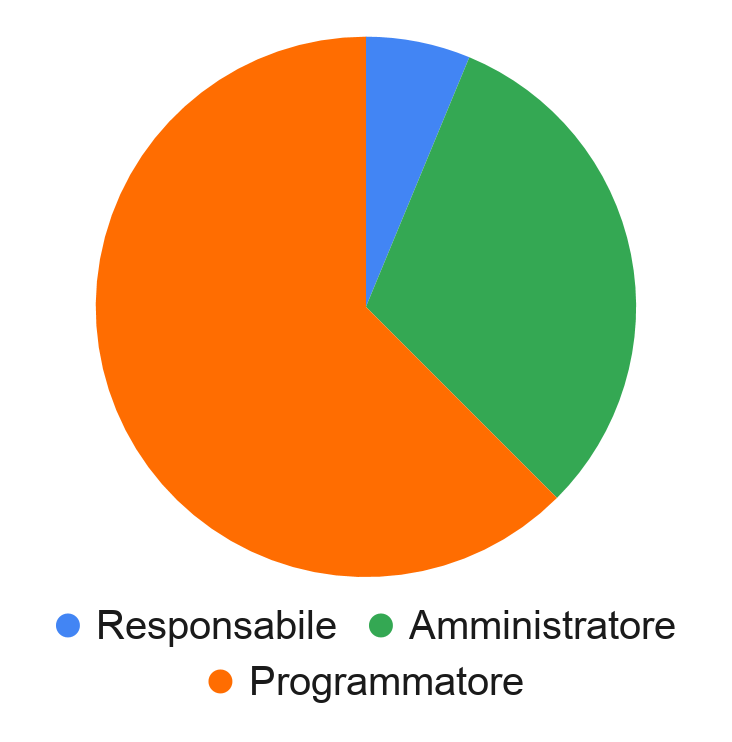
\includegraphics[scale=0.21]{res/images/charts/preventivo_priori/Grafico4-5.png}
	\caption{Distribuzione dei costi: preventivo - Progettazione Architetturale - Periodo 3}
\end{figure}
\end{minipage} 


\subsubsection{Pianificazione di periodo}


\begin{figure}[H]
	\centering
	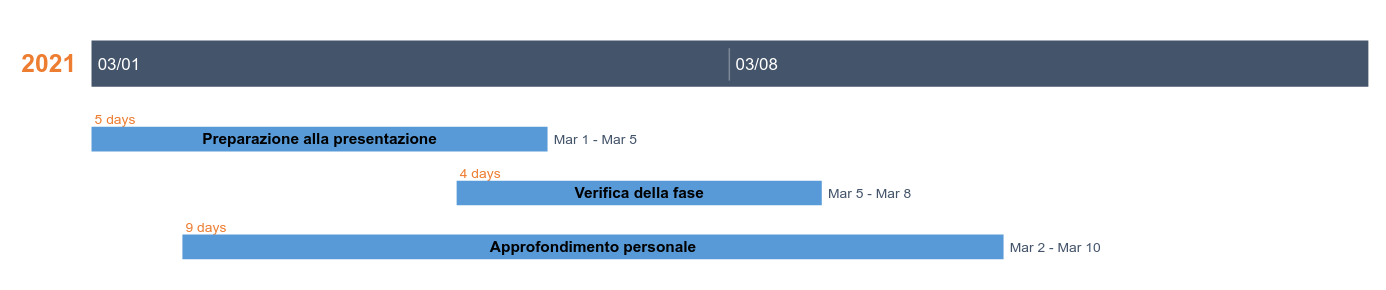
\includegraphics[scale=0.30]{res/images/gantt_periodo/progarch_3_gantt.png}
	\caption{Gantt di periodo\textsubscript{G} - Progettazione Architetturale - Periodo 3}
\end{figure}

\paragraph{Attività}
\subparagraph*{}

\planningTable{
	Preparazione alla presentazione & Viene preparato il materiale necessario alla presentazione & 5 & Amministratore
\tabularnewline 
Verifica dei macro periodi\textsubscript{G} precedenti & Il gruppo si vede coinvolto in un confronto dal quale vorranno emergere le criticità riscontrate nel macro periodo\textsubscript{G} trascorso, al fine di migliorare lo svolgimento dei periodi successivi. & 1 & Responsabile
\tabularnewline 
Approfondimento personale & Lo studio personale sarà rivolto alle tecnologie esplorate durante l'implementazione del Proof of Concept, al fine di raffinarne la comprensione e proporre un'implementazione migliorata nella codifica del software & 10 & Programmatore
\tabularnewline 
\caption{Pianificazione di periodo\textsubscript{G} - Progettazione Architetturale - Periodo 3}
}



\paragraph{Preventivo orario ed economico}
\subparagraph*{}

\contabilitaTable{
	Chiarello Sofia & 0 & 0 & 0 & 1 & 1 & 0 & \textbf{2}\\ 
Crivellari Alberto & 0 & 0 & 0 & 1 & 1 & 0 & \textbf{2}\\ 
De Renzis Simone & 1 & 0 & 0 & 0 & 0 & 0 & \textbf{1}\\ 
Greggio Nicolò & 0 & 0 & 0 & 1 & 1 & 0 & \textbf{2}\\ 
Tessari Andrea & 0 & 0 & 0 & 1 & 1 & 0 & \textbf{2}\\ 
Zuccolo Giada & 0 & 0 & 0 & 1 & 1 & 0 & \textbf{2}\\ 
\hlinetable 
\textbf{Totale orario} & \textbf{1} & \textbf{0} & \textbf{0} & \textbf{5} & \textbf{5} & \textbf{0} & \textbf{11}\\ 
\textbf{Totale costo} & \textbf{30} & \textbf{0} & \textbf{0} & \textbf{100} & \textbf{75} & \textbf{0} & \textbf{205}\\ 
\end{tabular} 
\caption{Preventivo di periodo - Progettazione Architetturale - Periodo 3}
}

\begin{figure}[H]
	\centering
	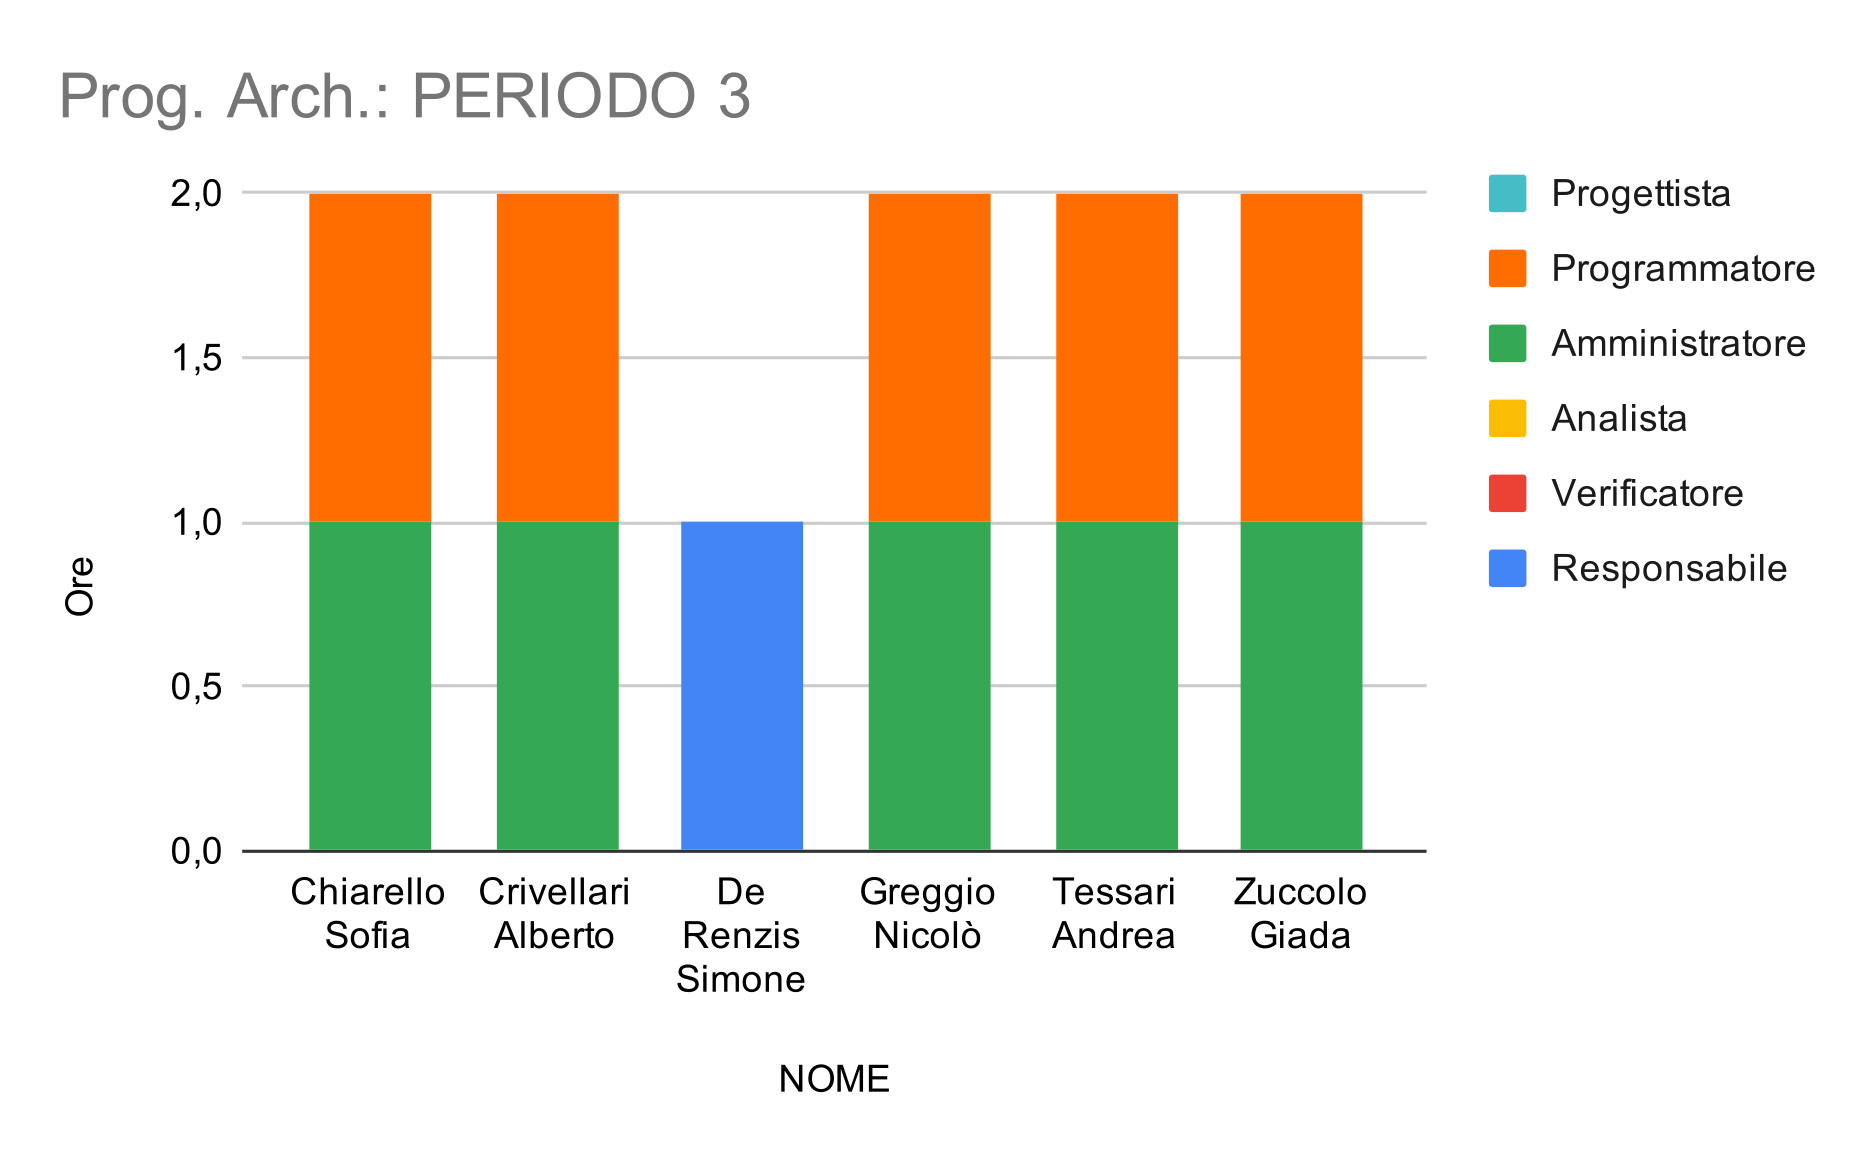
\includegraphics[scale=2]{res/images/charts/preventivo/prog_arch_3.png}
	\caption{Distribuzione oraria per componente: preventivo di periodo\textsubscript{G} - Progettazione Architetturale - Periodo 3}
\end{figure}

\subsubsection{Riscontro di fine periodo}


L'avanzamento del progetto\textsubscript{G} non prevede ancora la valorizzazione di questa sezione.